%%
%% Copyright 2019-2024 Elsevier Ltd
%%
%% This file is part of the 'CAS Bundle'.
%% --------------------------------------
%%
%% It may be distributed under the conditions of the LaTeX Project Public
%% License, either version 1.3c of this license or (at your option) any
%% later version.  The latest version of this license is in
%%    http://www.latex-project.org/lppl.txt
%% and version 1.3c or later is part of all distributions of LaTeX
%% version 1999/12/01 or later.
%%
%% The list of all files belonging to the 'CAS Bundle' is
%% given in the file `manifest.txt'.
%%
%% Template article for cas-dc documentclass for
%% double column output.

\documentclass[a4paper,fleqn]{cas-dc}

% If the frontmatter runs over more than one page
% use the longmktitle option.

%\documentclass[a4paper,fleqn,longmktitle]{cas-dc}

\usepackage[numbers]{natbib}
%\usepackage[authoryear]{natbib}
% \usepackage[authoryear,longnamesfirst]{natbib}
\usepackage{microtype}
\usepackage{xurl}
\usepackage{siunitx}
\usepackage{tabularx}
\usepackage{tikz}
\usetikzlibrary{positioning, arrows.meta, automata}

%%%Author macros
\def\tsc#1{\csdef{#1}{\textsc{\lowercase{#1}}\xspace}}
\tsc{WGM}
\tsc{QE}
%%%

% Uncomment and use as if needed
%\newtheorem{theorem}{Theorem}
%\newtheorem{lemma}[theorem]{Lemma}
%\newdefinition{rmk}{Remark}
%\newproof{pf}{Proof}
%\newproof{pot}{Proof of Theorem \ref{thm}}

\begin{document}
\let\WriteBookmarks\relax
\def\floatpagepagefraction{1}
\def\textpagefraction{.001}

% Short title
\shorttitle{BASE: Biometric Architecture for RTOS}

% Short author
\shortauthors{}

% Main title of the paper
\title [mode = title]{BASE: A Multi-Modal Biometric Architecture for Resource-Constrained RTOS}

% Title footnote mark
% eg: \tnotemark[1]
% \tnotemark[1]

% Title footnote 1.
% eg: \tnotetext[1]{Title footnote text}
% \tnotetext[1]{}

% First author
%
% Options: Use if required
% eg: \author[1,3]{Author Name}[type=editor,
%       style=chinese,
%       auid=000,
%       bioid=1,
%       prefix=Sir,
%       orcid=0000-0000-0000-0000,
%       facebook=<facebook id>,
%       twitter=<twitter id>,
%       linkedin=<linkedin id>,
%       gplus=<gplus id>]

\author[1,2]{Md~Siratul~Islam}[orcid=0009-0005-5945-8563]

% Footnote of the first author
\fnmark[1]

% Email id of the first author
\ead{email@sirat.me}

% URL of the first author
% \ead[url]{}

% Credit authorship
% eg: \credit{Conceptualization of this study, Methodology, Software}
\credit{Conceptualization, Methodology, Software, Writing}

% Address/affiliation
\affiliation[1]{organization={Department of Physics, Shahjalal University of Science and Technology},
            city={Sylhet},
            citysep={}, % Uncomment if no comma needed between city and postcode
            postcode={3114},
            state={Sylhet},
            country={Bangladesh}}

\author[2]{Md~Rasedujjaman}[orcid=0000-0002-8276-1860]

% Corresponding author indication
\cormark[1]

% Footnote of the second author
\fnmark[2]

% Email id of the second author
\ead{mrased-eee@sust.edu}

% URL of the second author
% \ead[url]{}

% Credit authorship
\credit{Supervision, Review \& Editing}

% Address/affiliation
\affiliation[2]{organization={Department of Electrical and Electronic Engineering, Shahjalal University of Science and Technology},
            city={Sylhet},
            citysep={}, % Uncomment if no comma needed between city and postcode
            postcode={3114},
            state={Sylhet},
            country={Bangladesh}}

% Corresponding author text
\cortext[1]{Corresponding author}

% Footnote text
% \fntext[1]{}

% For a title note without a number/mark
%\nonumnote{}

% Here goes the abstract
\begin{abstract}
Biometric authentication is replacing passwords in IoT devices, but developers face severe fragmentation as sensors ship with proprietary protocols and vendor-locked SDKs. They must choose between resource-heavy userspace frameworks unsuitable for microcontrollers or vendor-specific libraries that create hardware lock-in. We present the Biometric Abstraction for Secure Edge (BASE), the first dedicated kernel-level biometric subsystem for resource-constrained Real-Time Operating Systems. BASE decouples application logic from hardware specifics using driver-enforced state machines, standardized security attributes, and type-safe data structures. We validated BASE across three physical sensor families spanning contact fingerprint and camera-based multi-modal recognition (face and palm vein), with zero application code changes across all three. A minimum footprint of \SI{3.5}{\kilo\byte} Flash and \SI{644}{\byte} RAM confirms suitability for constrained MCUs. BASE has been merged into the Zephyr mainline kernel as the official biometrics subsystem.
\end{abstract}

% Use if graphical abstract is present
%\begin{graphicalabstract}
%\includegraphics{}
%\end{graphicalabstract}

% Research highlights
\begin{highlights}
\item A kernel-level biometric subsystem for resource-constrained RTOS.
\item Solves vendor lock-in across multi-modal biometric sensors.
\item Enforces deterministic enrollment state machines directly within the driver.
\item Enables zero-code-change app portability across various biometric sensor types.
\item Merged into Zephyr RTOS mainline as the official biometric subsystem.
\end{highlights}

%\nocite{*}

% Keywords
% Each keyword is seperated by \sep
\begin{keywords}
 IoT Security \sep Biometrics \sep Minimal Operating Systems \sep Device Software Development \sep Real-Time Operating Systems \sep Hardware Abstraction \sep Zephyr RTOS
\end{keywords}

\maketitle

% Main text
\section{Introduction}
\label{sec:introduction}

The Internet of Things (IoT) spans critical infrastructure, yet authentication mechanisms remain underdeveloped \cite{iotreview, ahvanooey2022modern} for resource-constrained edge devices. Widespread reliance on default credentials \cite{ibm2025} has pushed the industry toward inherence-based security (i.e., biometrics) \cite{markets2025}. However, despite this adoption, the integration landscape is severely fragmented; biometric modules ship with proprietary protocols, vendor-specific drivers, and mutually incompatible APIs \cite{yang2021biometric}.

Vendor fragmentation creates an architectural gap, particularly on resource-constrained microcontrollers. While high-level operating systems comply with standards like ISO/IEC 19784 (BioAPI) \cite{iso19784}, they lean on framework runtimes like D-Bus that require far more memory than a typical IoT end-node provides. ISO/IEC 29164 (Embedded BioAPI) \cite{iso29164} standardizes hardware interfaces at the wire-protocol level but specifies no host-side software behaviour. Developers are forced to write vendor-specific and non-portable code, which also results in inconsistent security policy enforcement.

This architectural gap is particularly evident in RTOS environments. Legacy approaches force developers to use generic sensor subsystems, forcing biometrics sensors to behave like passively read sensors, leaving enrollment state management entirely to the application layer, and cramming user identities into physics data structures. These limitations validate the need for a dedicated biometric subsystem that resolves type safety violations, stateless APIs applied to transactional workflows, and no focus on user management.

While legacy RTOS frameworks merely wrap bus transactions, to our knowledge, no existing solution offers a dedicated, kernel-level biometric abstraction. The fundamental novelty of the Biometric Abstraction for Secure Edge (BASE) lies in moving enrollment state machines (multi-step), type-safe data structures, and normalized security policies into a strict driver contract. By shifting this complexity into the kernel, BASE decouples application logic from hardware temporalities, enabling zero-code-change migrations across diverse sensor modalities. BASE is the first dedicated kernel-level biometric subsystem designed specifically for resource-constrained RTOS environments.

The specific contributions of this paper are:
\begin{itemize}
    \item \textbf{Kernel-Level Biometric Abstraction:} We propose BASE, a vendor-agnostic architecture that prevents type-safety violations and broken state management by enforcing a strict, deterministic enrollment state machine directly within the driver layer.
    \item \textbf{Strict Modality Independence:} We validated BASE across three different physical sensor families: contact-based optical fingerprint (ZFM-X0, GT-5X), and camera-based multi-modal recognition (DFRobot AI10, face and palm vein). The AI10 driver was developed by an independent contributor with zero modifications to the BASE API layer, confirming third-party implementability. Zero lines of application code changed across all three families.
    \item \textbf{Deterministic Multitasking:} BASE's API structures blocking operations around bounded timeouts. Empirical evaluation on an ARM Cortex-M4 shows BASE reduces maximum scheduling jitter from \SI{490}{\milli\second} to \SI{100}{\micro\second} and eliminates deadline misses entirely (0 vs.\ 68 out of 200) compared to a legacy blocking driver.
    \item \textbf{Industrial Standardization:} This architecture has been accepted by the Zephyr Architecture Working Group, merged into the mainline OS, and released as part of Zephyr 4.4\cite{zephyr_biometrics, zephyr_pr, zephyr_pr2, zephyr_44_notes}, where it is actively maintained by the first author.
\end{itemize}

The remainder of this paper is organized as follows: Section~\ref{sec:related_work} reviews related work. Section~\ref{sec:architecture} details the BASE architecture. Section~\ref{sec:implementation} describes the Zephyr integration. Section~\ref{sec:evaluation} presents the experimental results, and Section~\ref{sec:conclusion} concludes.

\section{Related Work and Motivation}
\label{sec:related_work}

\subsection{Biometric Authentication in IoT Systems}
Password-based authentication is insufficient and inefficient for resource-constrained IoT devices \cite{alotaibi2025}. Biometric authentication is a smart and efficient solution for IoT authentication. However, unlike passwords, a compromised biometric template cannot be reset \cite{edge2024}, which shifts the focus to encrypting biometric systems \cite{biosec2020}. Adapting these solutions to microcontrollers with limited RAM, however, remains a problem to be addressed\cite{acm2023}.

\subsection{Embedded Biometric Hardware Implementations}
Early fingerprint matching on 8-bit microcontrollers demonstrated possibilities but faced architectural challenges in generalizing across sensor types\cite{fons2012biometrics}. Template security, on the other hand, remained an active area, with works addressing encryption for template protection\cite{murillo2015robust} and fuzzy extractor schemes for key generation\cite{tran2024biometrics}. These works addressed algorithm and security concerns, but the software integration problem remained. This is what motivated this research.

\subsection{Software Integration Challenges}
\subsubsection{Fragmentation Across Ecosystems}
The biometric integration landscape is fragmented. Commercial SDKs exist but lock developers into proprietary APIs. Open-source implementations span single-threaded Arduino sketches to Linux-based systems, but each re-implements enrollment workflows from scratch\cite{mayron2015biometric}. The workflow incompatibility between two-step and three-step capture sequences forces per-sensor application logic. Academic prototypes on resource-rich platforms rely on full OS services\cite{restuccia2018survey} and ignore the multitasking and power constraints of RTOS systems. Recent surveys confirm this gap persists across IoT authentication research\cite{ahvanooey2022modern,yang2021biometric}. Table~\ref{tab:gap_matrix} evaluates representative approaches against the five integration requirements; no existing solution satisfies all five simultaneously.

\begin{table*}[!htbp]
\caption{Integration Gap Analysis Across Existing Approaches}
\label{tab:gap_matrix}
\centering
\renewcommand{\arraystretch}{1.3}
% This forces the table to shrink to exactly the width of the page
\resizebox{\textwidth}{!}{
\begin{tabular}{|c|c|c|c|c|c|c|}
\hline
\textbf{System} & \textbf{Architecture} & \textbf{RTOS-Aware} & \textbf{Type Safety} & \textbf{State Enforcement} & \textbf{Vendor Agnostic} & \textbf{MCU Constraints} \\
\hline
Linux fprintd\cite{linux_fprintd} & Userspace daemon, D-Bus IPC & No & High & OS-managed & Yes & No ($>$1 MB RSS) \\
\hline
Android BiometricPrompt\cite{android_bio} & Framework service, Binder IPC & No & High & OS-managed & Yes & No (MMU required) \\
\hline
ISO/IEC 29164\cite{iso29164} & Wire-protocol spec only & No & N/A & App responsibility & Partial & Partial \\
\hline
grow\_r502a\cite{zephyr_r502a} & Generic sensor adapter & Yes & Violated & App-managed flags & No & Yes \\
\hline
Arduino libs\cite{mayron2015biometric} & Blocking, single-threaded & No & Low & App-managed & No & Partial \\
\hline
\textbf{BASE (ours)} & \textbf{Kernel subsystem} & \textbf{Yes} & \textbf{Strict} & \textbf{Driver-enforced} & \textbf{Yes} & \textbf{Yes} \\
\hline
\end{tabular}
}
\end{table*}

\subsubsection{The Blocking I/O Antipattern}
We inspected vendor libraries (e.g., common Arduino fingerprint libraries) and found that they use busy-wait polling during the \num{200}--\SI{500}{\milli\second} image capture window, as shown in Figure~\ref{fig:blocking_comparison}. It is fine, as long as it is a single-threaded Arduino sketch. But in a multitasking RTOS, it blocks context switching \cite{zephyr_docs} and prevents the CPU from entering low-power idle states. This is a known inefficiency of blocking I/O in multitasking systems. The semaphore-based approach that BASE follows is standard RTOS driver practice.

\begin{figure}
\centering
\begin{scriptsize}
\begin{tabular}{p{0.45\columnwidth} | p{0.45\columnwidth}}
\textbf{A. Vendor Library Pattern} & \textbf{B. BASE Pattern (Ours)} \\
\hline
\begin{verbatim}
// Blocks CPU for ~500ms
while (get_image() != OK) {
   delay(100);
   // CPU cannot sleep
   // or switch tasks
}
\end{verbatim}
&
\begin{verbatim}
// Yields CPU to Scheduler
// Blocks only calling thread
if (k_sem_take(&sem,
      K_MSEC(500)) != 0) {
   return -ETIMEDOUT;
}
\end{verbatim}
\\
\end{tabular}
\end{scriptsize}
\caption{Comparison of polling mechanisms. Vendor libraries (A) busy-wait, which prevents power-saving states. BASE (B) uses RTOS semaphores and cooperative yielding to release the CPU during sensor latency.}
\label{fig:blocking_comparison}
\end{figure}

\subsection{Standardization Landscape}
\subsubsection{High-Level Standards (ISO/IEC 19784)}
 Linux \textit{fprintd} \cite{linux_fprintd} and Android BiometricPrompt \cite{android_bio} use the framework defined by ISO/IEC 19784 (BioAPI) \cite{iso19784}. The drawback is that they both rely on heavy IPC mechanisms, D-Bus on Linux, Binder on Android. It also assumes a memory-managed environment with MMUs and $>$\SI{1}{\mega\byte} RAM, which leaves a microcontroller with \SI{128}{\kilo\byte} total RAM and no MMU out of consideration.

\subsubsection{Embedded Standards (ISO/IEC 29164)}
ISO/IEC 29164 (Embedded BioAPI) \cite{iso29164} targets constrained devices and does its job well at the wire-protocol level. It defines the command encoding and message framing between host and biometric module but it does not specify host-side elements, such as concurrency handling, enrollment state management, or power management. This leaves the responsibility to the application developer. For a single-sensor, single-threaded project this is workable. For a multitasking RTOS deployment across heterogeneous sensors, it is not.

\subsection{Inadequacy of Generic Sensor Subsystems}
\label{sec:sensor_limitations}

When we tried to develop a fingerprint sensor driver for Zephyr, our closest solution was to use the Sensor API. But it was not straightforward and required a lot of workarounds to get basic functionalities working. This is when we felt the need for a dedicated subsystem for biometrics. We looked at the existing \texttt{grow\_r502a} driver \cite{zephyr_r502a} and found the following architectural issues that application-level workarounds cannot resolve.

\subsubsection{Semantic Mismatch and Type Safety Violations}
The sensor API defines structures for physical measurements-\texttt{sensor\_value.val1}, \texttt{sensor\_value.val2} representing temperature or acceleration \cite{zephyr_sensor_api}. The \texttt{grow\_r502a} driver used these for storing user IDs or for template count, inconsistently \cite{zephyr_r502a_sample}. It treated a security principal as if it were a temperature reading. A lack of standardization also meant users must know the driver code to use it. This was not a flexible choice of the driver but forced by the API's data model. Any biometric driver built on the sensor subsystem hits this same wall, and the compiler cannot catch it because a user ID and a temperature reading are both just integers.

\subsubsection{Stateless vs. Transactional Workflows}
The sensor subsystem assumes a stateless fetch-and-get cycle \cite{zephyr_sensor_api}. Repeated reads return idempotent values, that is the general assumption. Whereas the biometric enrollment process is the opposite. It is a strict sequence (Start $\rightarrow$ Capture $\rightarrow$ Merge $\rightarrow$ Finalize) where each step depends on the previous one. Fitting this into a stateless API meant the application had to manage the state machine manually using flags \cite{zephyr_r502a}, and discarding driver abstraction entirely \cite{zephyr_driver}. It will be even worse, if the application calls steps out of order, or skips one, the sensor returns an error with no indication of which step failed which may leave the application in an undefined state.

\subsubsection{Leaky Abstractions}
The driver exposes operations through hardware-specific attributes like \texttt{SENSOR\_ATTR\_R502A\_RECORD\_DEL} through hardware-specific public headers. This clutters the OS as well as requires application code to include very specific headers like \texttt{<drivers/sensor/grow\_r502a.h>} \cite{zephyr_r502a}. Swap the sensor, and the application breaks. This is the textbook definition of a leaky abstraction \cite{zephyr_driver}, and it exists because the sensor subsystem was never designed for biometric workflows.

\subsection{Summary: The Integration Gap}
As Table~\ref{tab:gap_matrix} shows, every existing approach fails on at least two of the five requirements. Heavy userspace services handle type safety and vendor agnosticism but cannot run on MCUs. Generic sensor adapters run on MCUs but violate type safety and push state management to the application. No existing solution enforces transactional state at the driver level while satisfying MCU memory constraints. We translated these three failure modes into design requirements: strict biometric types enforced at the kernel level, driver-level state machines for enrollment workflows, and vendor-neutral attribute interfaces for security policy. For the reference implementation we chose Zephyr due to its subsystem architecture, Linux Foundation backing, and active industrial adoption. Section~\ref{sec:architecture} presents BASE's architecture around these requirements.
\section{The BASE Architecture}
\label{sec:architecture}

We designed BASE to directly address the integration barriers identified in Section~\ref{sec:sensor_limitations}. It eliminates type-safety violations, resolves broken state management by moving sequencing into the kernel, and repairs leaky abstractions by isolating all vendor-specific protocol details. By integrating these solutions as a dedicated RTOS subsystem, BASE enforces secure, deterministic behavior by default.

\subsection{Three-Plane Architecture}

BASE separates concerns across three layers (Figure~\ref{fig:architecture}). The Application Plane provides unified enrollment and matching interfaces via standard RTOS system calls. The Subsystem Contract Plane normalizes hardware capabilities, enforces type safety, and abstracts protocol-specific details. The Driver Implementation Plane isolates all vendor-specific UART/SPI protocols and sensor state. No layer reaches past its boundary.

\begin{figure*}
    \centering
    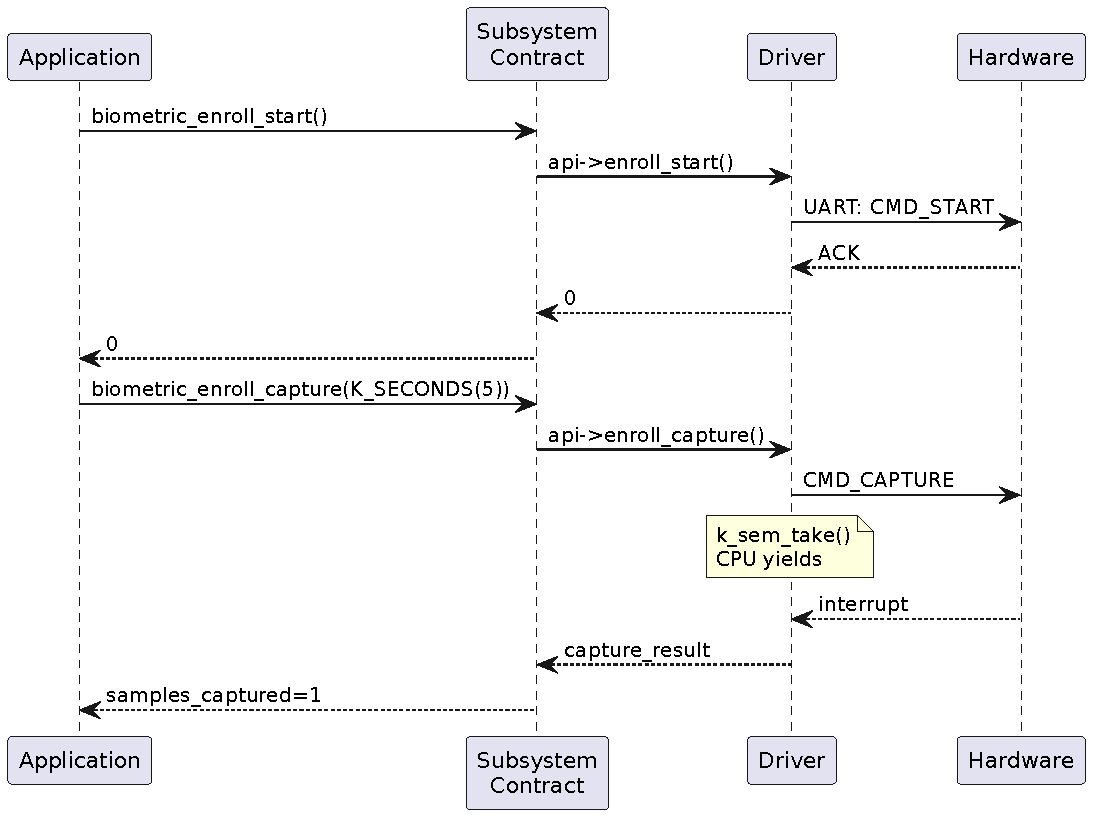
\includegraphics[width=\textwidth]{figs/fig_architecture.pdf}
    \caption{Three-plane architecture of BASE. The contract plane dispatches to three driver families spanning contact fingerprint (ZFM-X0, GT-5X) and camera-based multi-modal sensing (AI10). No layer reaches past its boundary.}
    \label{fig:architecture}
\end{figure*}

The Application Plane provides unified enrollment, matching, and template management interfaces. Applications never access hardware drivers directly. All public functions are defined via standard RTOS system calls (e.g., Zephyr's \texttt{\_\_syscall} annotation, which generates kernel-mode dispatch for each entry point), allowing the driver to run in privileged mode while the application runs in userspace. On POSIX-compliant systems such as NuttX, the same boundary is enforced via VFS \texttt{ioctl()} calls; on capability-based systems such as TockOS, via capsule syscalls. This protects the biometric state machine from application-level crashes or memory corruption. Errors are indicated by standard POSIX error codes (i.e., EBUSY, EINVAL).

The Subsystem Contract Plane defines the \\ \texttt{biometric\_driver\_api} structure that biometric drivers are required to implement. This layer normalizes different hardware capabilities into standardized attribute enumerations. It also abstracts away protocol-specific endianness. Applications work without the knowledge of whether a sensor communicates in Big Endian (ZFM-70) or Little Endian (GT-521F32).

The Driver Implementation Plane consists of hardware drivers that comply with the requirements of the Contract Plane. These drivers handle the low-level communication protocols (e.g., UART packet framing, checksum calculation) and manage the sensor's physical state. By isolating these details at the bottom of the stack, BASE ensures that protocol-level changes such as switching from a packet-based ZFM sensor to a command-based GT-5X sensor remain transparent to the higher layers. It is also possible to integrate Trusted Execution Environment (TEE), where matching logic can be further offloaded to secure zones like ARM TrustZone.

\subsection{API Specification}

\subsubsection{Core Data Types}

We defined five core types based on biometric concerns: capabilities, match outcomes, enrollment progress, policy configuration, and on-device user metadata. This allowed us to replace the legacy behavior of forcing user IDs, template count, and score into \texttt{sensor\_value} fields (Table~\ref{tab:data_types}). This is the type safety that the generic sensor API cannot provide.

\begin{table}
\caption{BASE Core Data Types}
\label{tab:data_types}
\centering
\renewcommand{\arraystretch}{1.4}
\setlength{\tabcolsep}{5pt}
\begin{tabularx}{\columnwidth}{|l|X|}
\hline
\textbf{Type} & \textbf{Purpose} \\
\hline
\texttt{biometric\_capabilities} & Hardware features: \texttt{supported\_modalities} bitmask (multi-modal), max templates, samples required, storage modes \\
\hline
\texttt{biometric\_match\_result} & Match outcome: confidence, template ID, quality (0--100), \texttt{modality} field identifying which sensing modality produced the result \\
\hline
\texttt{biometric\_capture\_result} & Enrollment progress: samples captured/required, quality, assigned template ID \\
\hline
\texttt{biometric\_attribute} & Config: match thresholds, security levels, timeouts, duplicate enrollment policy \\
\hline
\texttt{biometric\_user\_info} & On-device user metadata: name string, privilege level \\
\hline
\end{tabularx}
\end{table}

\subsubsection{Enrollment and Match APIs}
Enrollment abstracts the varying sample counts across hardware (e.g., 2 for ZFM, 3 for GT-5X, 1 for AI10). Applications repeatedly call \texttt{biometric\_enroll\_capture()} until \texttt{samples\_required} is met, then call \texttt{biometric\_enroll\_finalize()}. Similarly, the Match API hides hardware-specific search optimizations behind a unified \texttt{biometric\_match()} interface that supports both 1:1 verification and 1:N identification.

\subsubsection{API Correctness Contracts}

We specify the behavioral obligations of BASE drivers using Hoare triple notation $\{P\}\;C\;\{Q\}$, where $P$ is the precondition and $Q$ the postcondition for operation $C$. $\mathtt{stored}(\mathit{id})$ denotes template $\mathit{id}$ is persistently committed; $\mathtt{exists}(\mathit{dev},\mathit{id})$ denotes it is present; $\mathrm{DB}$ is the set of enrolled templates.

\paragraph{Enrollment start:}
\begin{multline}
  \{\mathrm{state} = q_{\mathrm{idle}}\}\;\;
  \mathtt{enroll\_start}(\mathit{dev},\,\mathit{id})\;\; \\
  \{\mathrm{state} = q_{\mathrm{w},1} \;\wedge\; \mathtt{enrolled\_id} = \mathit{id}\}
\end{multline}

\paragraph{Sample capture:} For $1 \le k \le N$, with $\sigma$
the outcome symbol (\texttt{capture\_ok} or \texttt{capture\_fail}) corresponding to the return value:
\begin{multline}
  \{\mathrm{state} = q_{\mathrm{w},k}\}\;\;
  \mathtt{enroll\_capture}(\mathit{dev},\,t,\,\&r)\\
  \{\mathrm{state} = \delta(q_{\mathrm{w},k},\,\sigma)\}
\end{multline}

\paragraph{Template finalization:}
Here $\mathit{id}$ is the logical variable bound by the preceding $\mathtt{enroll\_start}(\mathit{dev},\,\mathit{id})$ call.
\begin{multline}
  \{\mathrm{state} = q_{\mathrm{ready}}
   \;\wedge\; \mathtt{enrolled\_id} = \mathit{id}\}\;\; \\
  \mathtt{enroll\_finalize}(\mathit{dev})\\
  \{\mathrm{state} = q_{\mathrm{idle}}
   \;\wedge\; \mathtt{stored}(\mathit{id})\}
\end{multline}

\paragraph{Match non-interference.}
\begin{multline}
  \{\mathrm{DB} = \mathrm{DB}_0\}\;\;
  \mathtt{match}(\mathit{dev},\,\mathit{mode},\,\mathit{id},\,t,\,\&r)\\
  \{\mathrm{DB} = \mathrm{DB}_0\}
\end{multline}

\paragraph{Template deletion.}
\begin{multline}
  \{\mathtt{exists}(\mathit{dev},\,\mathit{id})\}\;\;
  \mathtt{template\_delete}(\mathit{dev},\,\mathit{id})\;\; \\
  \{\neg\,\mathtt{exists}(\mathit{dev},\,\mathit{id})\}
\end{multline}


\subsubsection{Auxiliary Match Output}
Sensor-specific auxiliary output, such as liveness score blobs or custom data, would either pollute \\ \texttt{biometric\_match\_result} with union fields, breaking type safety, or require sensor-specific calls, breaking the abstraction. \texttt{biometric\_match\_get\_data()} resolves this: a standardized optional side-channel, null-guarded, with a defined retrieval window (must be called before the next match operation). Rich sensor output flows through a typed buffer without contaminating the universal result structure.

\subsubsection{Portable Security Configuration}
Security parameters (Table~\ref{tab:attributes}) map normalized 0--100/1--10 ranges to hardware-specific values via \texttt{biometric\_attr\_set()}. This enables zero-code-change policy portability, allowing seamless hardware swapping without altering application compliance logic.

\begin{table}
\caption{Security Configuration Attributes}
\label{tab:attributes}
\centering
\renewcommand{\arraystretch}{1.4}
\setlength{\tabcolsep}{4pt}
\begin{tabularx}{\columnwidth}{|l|c|X|}
\hline
\textbf{Attribute} & \textbf{Range} & \textbf{Function} \\
\hline
\texttt{MATCH\_THRESHOLD} & 0--100 & Min similarity score (\%) \\
\hline
\texttt{SECURITY\_LEVEL} & 1--10 & FAR (False Accept Rate) control \\
\hline
\texttt{ENROLL\_QUALITY} & 0--100 & Min image quality \\
\hline
\texttt{TIMEOUT\_MS} & 0--3.6M & Max operation timeout (ms) \\
\hline
\texttt{ANTI\_SPOOF} & 1--10 & Liveness detection sensitivity \\
\hline
\texttt{IMAGE\_QUALITY} & read-only & Last captured sample quality score \\
\hline
\texttt{DUPLICATE\_POLICY} & 0--1 & Reject (0) or allow (1) duplicate enrollments \\
\hline
\end{tabularx}
\end{table}

A sensor supporting 1--5 security levels maps the subsystem's 1--10 scale via \texttt{hw\_level = CLAMP((val+1)/2, 1, 5)}. An application that sets 80\% match threshold and security level 8 gets those exact values regardless of which sensor is on the board. The hardware can be easily swapped with no change in the policy. This increases accessibility and portability in security-critical deployments like payment terminals, medical device access control, industrial safety interlocks etc. It also supports compliance with NIST SP 800-63B \cite{nist_800_63b}, which requires specific False Accept Rates based on the authentication assurance level. Auditors can inspect devicetree bindings or application configuration to verify compliance without looking at the driver internals. For hardware-specific parameters, the enum reserves \texttt{BIOMETRIC\_ATTR\_PRIV\_START} and above for driver-private attributes, accessible through the same \texttt{biometric\_attr\_set()} interface without requiring sensor-specific headers in application code. The attribute-based security model aligns with contemporary recommendations for IoT device authentication\cite{wu2023attacks,sicari2015security}.

\begin{figure*}
    \centering
    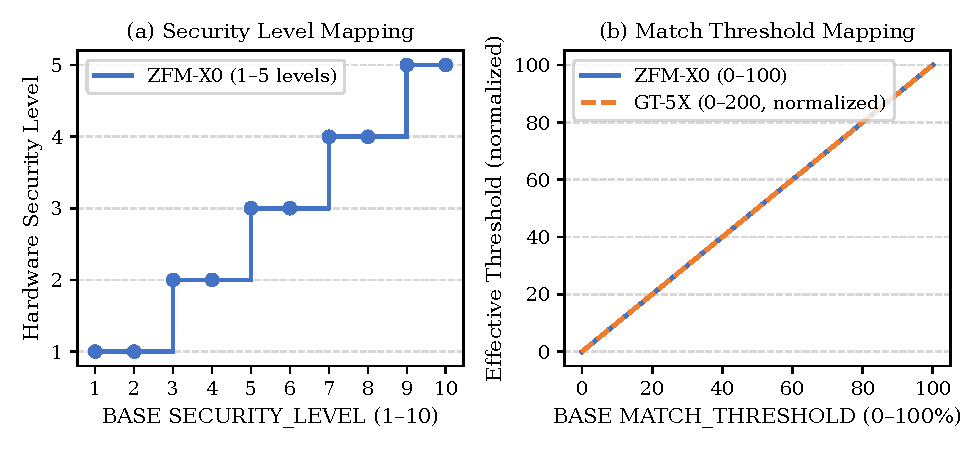
\includegraphics[width=\textwidth]{figs/fig_normalization.pdf}
    \caption{Attribute normalization mapping curves.}
    \label{fig:normalization}
\end{figure*}

\subsection{Enrollment State Machine}

To guarantee deterministic behavior, BASE mandates a strict enrollment state machine via the MUST contract. We formalize this as a Deterministic Finite Automaton $\mathcal{A} = (Q, \Sigma, \delta, q_0, F)$. \\

\noindent\textbf{States.} For a sensor requiring $N$ samples:
\begin{equation}
  Q = \{q_{\mathrm{idle}},\;
        q_{\mathrm{w},1},\; \ldots,\; q_{\mathrm{w},N},\;
        q_{\mathrm{ready}}\}
  \label{eq:states}
\end{equation}
$q_{\mathrm{idle}}$: subsystem inactive. $q_{\mathrm{w},k}$: enrollment active, $k{-}1$ samples captured, awaiting the $k$-th. $q_{\mathrm{ready}}$: all $N$ samples captured; driver authorized to commit the template. \\

\noindent\textbf{Input alphabet:}
\begin{multline}
  \Sigma = \{\mathtt{start},\;
             \mathtt{capture\_ok},\;
             \mathtt{capture\_fail},\; \\
             \mathtt{finalize},\;
             \mathtt{abort}\}
  \label{eq:alphabet}
\end{multline}

\noindent\textbf{Transition function:}
\begin{align}
  \delta(q_{\mathrm{idle}},\; \mathtt{start})
    &= q_{\mathrm{w},1}
    \label{eq:d_start}\\
  \delta(q_{\mathrm{w},k},\; \mathtt{capture\_ok})
    &= q_{\mathrm{w},k+1},
    \quad 1 \le k < N
    \label{eq:d_ok}\\
  \delta(q_{\mathrm{w},N},\; \mathtt{capture\_ok})
    &= q_{\mathrm{ready}}
    \label{eq:d_final}\\
  \delta(q_{\mathrm{w},k},\; \mathtt{capture\_fail})
    &= q_{\mathrm{w},k},
    \quad 1 \le k \le N
    \label{eq:d_fail}\\
  \delta(q_{\mathrm{ready}},\; \mathtt{finalize})
    &= q_{\mathrm{idle}}
    \label{eq:d_finalize}\\
  \delta(q,\; \mathtt{abort})
    &= q_{\mathrm{idle}},
    \quad \forall\, q \in Q \setminus \{q_{\mathrm{idle}}\}
    \label{eq:d_abort}
\end{align}

Any $(q, \sigma)$ pair not listed above leaves the state unchanged; the API call returns \texttt{-EINVAL}, with the exception that $\delta(q_{\mathrm{idle}},\,\mathtt{abort})$ returns \texttt{-EALREADY}, distinguishing the ``already idle'' condition from a malformed call. Initial state $q_0 = q_{\mathrm{idle}}$; accepting state $F = \{q_{\mathrm{ready}}\}$. Figure~\ref{fig:fsm} illustrates $\mathcal{A}$ for $N = 2$.

\begin{proposition}[No Partial Template Storage]
\label{prop:safety}
For any execution trace $\tau \in \Sigma^*$, a template is committed to persistent storage only after exactly $N$ $\mathtt{capture\_ok}$ events following the most recent $\mathtt{start}$ event.
\end{proposition}

\begin{proof}
Template storage is triggered exclusively by \\ $\delta(q_{\mathrm{ready}},\,\mathtt{finalize}) = q_{\mathrm{idle}}$ (Eq.~\eqref{eq:d_finalize}), which is defined only when the current state is $q_{\mathrm{ready}}$. For all $q \neq q_{\mathrm{ready}}$, the pair $(q,\, \mathtt{finalize})$ is undefined; the API returns \texttt{-EINVAL} and the state is unchanged. By Eq.~\eqref{eq:d_final}, $q_{\mathrm{ready}}$ is the unique target of $\delta(q_{\mathrm{w},N},\,\mathtt{capture\_ok})$. By induction on $k$ using Eq.~\eqref{eq:d_ok}: state $q_{\mathrm{w},k}$ is reachable only after exactly $k$ $\mathtt{capture\_ok}$ events since the last $\mathtt{start}$; $\mathtt{capture\_fail}$ self-loops (Eq.~\eqref{eq:d_fail}) do not advance $k$. Therefore $q_{\mathrm{ready}}$ requires exactly $N$ $\mathtt{capture\_ok}$ events. This is enforced in each reference driver by:
\begin{verbatim}
  if (data->enroll_state != ENROLL_READY)
      return -EINVAL;
\end{verbatim}
\end{proof}

\begin{figure}
    \centering
    \resizebox{\columnwidth}{!}{%
        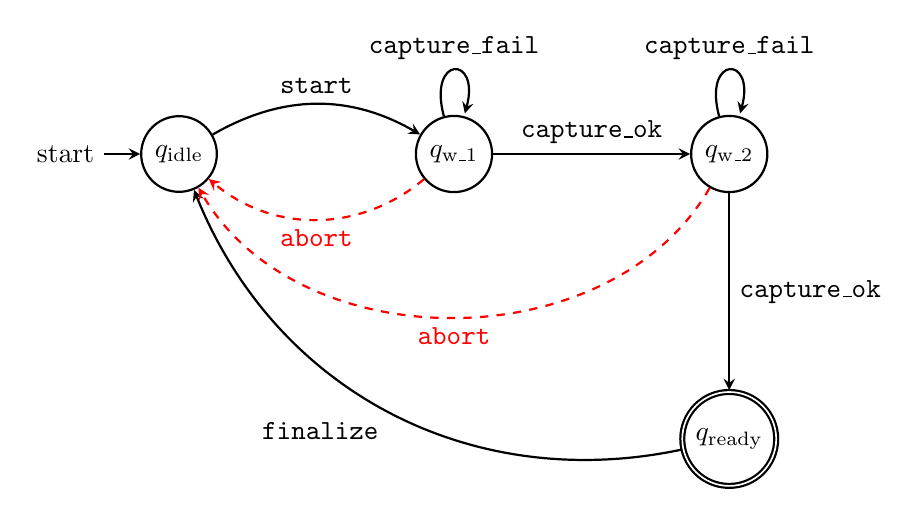
\begin{tikzpicture}[->, >=stealth, node distance=2.5cm, auto, thick]
            \node[state, initial] (idle) {$q_{\mathrm{idle}}$};
            \node[state] (wait1) [right=of idle] {$q_{\mathrm{w\_1}}$};
            \node[state] (wait2) [right=of wait1] {$q_{\mathrm{w\_2}}$};
            \node[state, accepting] (ready) [below=of wait2] {$q_{\mathrm{ready}}$};

            \path
            (idle) edge [bend left] node {\texttt{start}} (wait1)
            (wait1) edge [loop above] node {\texttt{capture\_fail}} (wait1)
            (wait1) edge node {\texttt{capture\_ok}} (wait2)
            (wait2) edge [loop above] node {\texttt{capture\_fail}} (wait2)
            (wait2) edge node {\texttt{capture\_ok}} (ready)
            (ready) edge [bend left=40] node {\texttt{finalize}} (idle);

            \path[dashed, color=red]
            (wait1) edge [bend left=40] node[below] {\texttt{abort}} (idle)
            (wait2) edge [bend left=60] node[below] {\texttt{abort}} (idle);

        \end{tikzpicture}%
    }
    \caption{State transition diagram for BASE enrollment workflow (Case $N=2$).}
    \label{fig:fsm}
\end{figure}

\subsection{Interrupt-Driven I/O and Power Efficiency}
\label{sec:interrupt_io}

Legacy vendor libraries busy-wait during the \num{200}--\SI{500}{\milli\second} sensor capture window, keeping the CPU at full clock speed and preventing the scheduler from running other threads. BASE addresses this at two levels.

At the \textbf{API level}, every blocking operation accepts a \texttt{k\_timeout\_t} parameter, making bounded blocking a contract requirement rather than a convention. This enables application-level deadline analysis without inspecting driver internals. For sensors supporting hardware-triggered recognition, BASE provides the functions \texttt{biometric\_match\_start()} and \texttt{biometric\_match\_stop()} with a registered callback handler, forming a complete async matching interface. The driver manages the recognition loop internally and invokes the callback per result, decoupling recognition events from the application thread.

At the \textbf{driver level}, all UART transactions in the reference drivers are interrupt-driven via binary semaphores. On sensors without a hardware finger-detect interrupt (ZFM-X0, GT-5X), presence detection uses \texttt{k\_msleep}-based cooperative polling between queries. In all cases the calling thread yields the CPU throughout the capture window. This is validated empirically in Section~\ref{sec:eval_concurrency}.

\subsection{Driver Implementation Contract}

The driver contract uses three compliance tiers enforced by the API structure itself. \textbf{MUST} functions (six total: \texttt{get\_capabilities}, \texttt{enroll\_start}, \texttt{enroll\_capture}, \\ \texttt{enroll\_finalize}, \texttt{match}, \texttt{template\_delete}) are called unconditionally in their \texttt{z\_impl} wrappers; an unimplemented MUST function crashes at runtime. \textbf{SHOULD} functions cover template management, policy configuration, enrollment abort, async matching (\texttt{match\_set\_cb}, \texttt{match\_start}, \texttt{match\_stop}), auxiliary output (\texttt{match\_get\_data}), and user metadata; these return \texttt{-ENOSYS} if unimplemented. \textbf{MAY} functions cover hardware-dependent features such as LED control and image-based enrollment. The distinction is enforced by null guards in the subsystem header, not by convention.

\subsection{Real-Time and Resource Analysis}

All host-side operations maintain $O(1)$ time and space complexity; 1:N identification complexity resides within the sensor hardware. The schedulability impact of BASE's yielding I/O model is evaluated empirically in Section~\ref{sec:eval_concurrency}.

The host-side enrollment workflow executes a fixed sequence of $N$ API calls regardless of database size; $N$ is bounded by \texttt{max\_templates}. Match and delete perform a fixed number of UART transactions per operation. Thus all host-side operations are $O(1)$ in time and space with respect to enrolled template count.

Under Rate Monotonic Scheduling with $\tau_1$ ($T_1=10\,\text{ms}$, $C_1 \leq 50\,\mu\text{s}$, conservative upper bound on the loop body executing \texttt{k\_uptime\_ticks()} plus deadline comparison) and $\tau_2$ ($T_2=500\,\text{ms}$, one sensor capture period; $C_2=0.05\,\text{ms}$, derived from the $100\,\mu\text{s}$ measured scheduling overhead under BASE), CPU utilization is:
\begin{equation}
  U = \frac{C_1}{T_1} + \frac{C_2}{T_2}
    = \frac{0.05}{10} + \frac{0.05}{500}
    = 0.005 + 0.0001 \approx 0.005
\end{equation}

The Liu--Layland bound for $n=2$ tasks is $U \leq 2(2^{1/2}-1) \approx 0.83$. Since $0.005 \ll 0.83$, schedulability is guaranteed with a ${\sim}160\times$ margin, confirming the empirical results in Section~\ref{sec:eval_concurrency}.

\subsection{Security and Threat Model}
\label{sec:threat_model}
BASE may mitigate several attack vectors inherent to edge biometrics:
\begin{itemize}
    \item \textbf{Application Bug Exploitation:} Kernel-space driver isolation prevents an exploited userspace thread from locking the sensor state or bypassing authentication timeouts.
    \item \textbf{Partial Enrollment Injection:} The deterministic driver state machine rejects incomplete capture sequences, preventing attackers from injecting partial or corrupted templates into the database.
    \item \textbf{Command Bypasses:} Applications cannot send arbitrary raw hex commands directly to the hardware bus, mitigating undocumented backdoor access to the sensor firmware.
    \item \textbf{Duplicate Enrollment:} The subsystem exposes a configurable duplicate enrollment policy, allowing operators to reject duplicate biometric registrations at the driver level and prevent identity aliasing attacks.
\end{itemize}

\subsection{OS-Agnostic Paradigm Mapping}
\label{sec:os_agnostic}
While we selected Zephyr for our reference implementation (Section~\ref{sec:implementation}), BASE's three-plane architecture is fundamentally OS-agnostic. By abstracting the enrollment state machine and data types into a strict contract, BASE maps cleanly to diverse embedded OS paradigms:
\begin{itemize}
    \item \textbf{POSIX-Compliant (e.g., Apache NuttX):} The Subsystem Contract Plane maps directly to the Virtual File System (VFS) as a character device (\texttt{/dev/biometric0}), utilizing standard \texttt{ioctl()} commands to configure security attributes.
    \item \textbf{Device Frameworks (e.g., RT-Thread):} The architecture translates natively to an \texttt{rt\_device} class, encapsulating the state machine behind standard \texttt{rt\_device\_read()} and \texttt{rt\_device\_control()} interfaces.
    \item \textbf{Capability-Based (e.g., TockOS):} BASE's state machine can be encapsulated as a trusted kernel capsule. The Application Plane interacts via asynchronous system calls (grants and upcalls) to guarantee strict memory safety between the kernel and untrusted userspace.
\end{itemize}
By enforcing correctness at the architectural level rather than the kernel level, BASE ensures that its core security and schedulability guarantees remain intact regardless of the host operating system's design philosophy.

The reference implementation uses only three primitive categories: mutex, binary semaphore, and monotonic timeout, each of which maps directly to equivalents in NuttX, RT-Thread, TockOS, and bare-metal systems, confirming that porting BASE requires no architectural changes.

\subsection{Distinction from Generic Driver Models}

Although the three-plane design resembles layered driver models in Zephyr's sensor subsystem or Linux IIO, BASE's contract plane is fundamentally different: it is an \emph{active behavioral enforcer}. Generic subsystems only define a vtable and treat operations as stateless. BASE's contract plane mandates that drivers implement the enrollment state machine via the MUST contract. Each reference driver enforces the ready-state guard internally before committing a template. A driver that skips this guard violates the BASE contract and fails compliance. This architectural separation, subsystem defines the invariant, driver enforces it, is what distinguishes BASE from a generic vtable.
\section{Implementation}
\label{sec:implementation}

\subsection{Zephyr RTOS Integration}

The subsystem header (\texttt{drivers/biometrics.h}) defines the public API using static inline wrappers. Each public API function carries the \texttt{\_\_syscall} annotation, triggering kernel-mode dispatch code generation per entry point.

\begin{table}
\caption{Implementation Metrics (WeAct STM32F446RE)}
\label{tab:implementation_metrics}
\centering
\renewcommand{\arraystretch}{1.3}
\begin{tabularx}{\columnwidth}{|X|c|c|c|}
\hline
\textbf{Component} & \textbf{Flash (B)} & \textbf{Static RAM (B)} & \textbf{Heap (B)} \\
\hline
BASE Core API & 0 (Inlined) & 0 & 0 \\
\hline
ZFM-X0 Driver & 3,514 & 644 & 0 \\
\hline
GT-5X Driver & 4,288 & 144 & $\sim$520 \\
\hline
AI10 Driver & 4,974 & 2,176 & 0 \\
\hline
Typical Config & $<$ \SI{5}{\kilo\byte} & $<$ \SI{3}{\kilo\byte} & $<$ \SI{1}{\kilo\byte} \\
\hline
\end{tabularx}
\vspace{2pt}
\footnotesize{\\ \textit{Note: GT-5X uses dynamic allocation for packet buffers; ZFM-X0 and AI10 use static buffers. AI10 RAM includes dual frame buffers and continuous match thread state. AI10 figures reflect a pre-upstream implementation; the driver is under active development and footprint may change prior to merge.}}
\end{table}

\subsection{Driver Implementations}

\subsubsection{ZFM-X0 Family Driver}

The ZFM-X0 driver targets the ZhianTec protocol family (ZFM-20/60/70 and rebrands including Adafruit, Grow R307, and Hi-Link capacitive modules). It uses a variable-length packet format with checksum validation and fully interrupt-driven UART communication via semaphores. The driver enforces the four-state enrollment machine and supports both optical and capacitive sensors with identical code.

\subsubsection{GT-5X Family Driver}

The GT-5X driver targets the ADH-Tech optical family (GT-511C3/521F32/521F52). It implements the fixed 12-byte command protocol with 29 opcodes. The driver uses dynamic allocation only for packet buffers while satisfying the $O(1)$ memory contract and requires three samples for enrollment.

\subsubsection{DFRobot AI10 Driver (Multi-Modal)}

The AI10 driver targets the DFRobot SEN0677 module, a binocular camera-based sensor supporting face recognition and palm vein detection on a single device. This is the first driver in the BASE ecosystem to demonstrate the multi-modal capability: \texttt{get\_capabilities()} reports \texttt{supported\_modalities = BIOMETRIC\_MODALITY\_FACE | BIOMETRIC\_MODALITY\_PALM}. The driver maps face UIDs (1--1000) and palm UIDs (1001--2000) transparently into the standard \texttt{biometric\_match\_result} structure by setting the \texttt{modality} field accordingly. Enrollment uses a single-shot command, but the application loop remains identical across all drivers because it checks \texttt{samples\_required} (set to 1 for AI10).

\subsubsection{Protocol Comparison}

Table~\ref{tab:protocol_comparison} summarizes the three driver families.

\begin{table*}[!ht]
\caption{Driver Protocol Comparison}
\label{tab:protocol_comparison}
\centering
\renewcommand{\arraystretch}{1.2}
\setlength{\tabcolsep}{4pt}
\begin{tabularx}{\textwidth}{|l|X|X|X|}
\hline
\textbf{Feature} & \textbf{ZFM-X0} & \textbf{GT-5X} & \textbf{DFRobot AI10} \\
\hline
Sensor Type & Optical/Capacitive contact & Optical contact & Camera-based, binocular \\
\hline
Modalities & Fingerprint & Fingerprint & Face + Palm vein \\
\hline
Start Code & \texttt{0xEF01} & \texttt{0x55AA}/\texttt{0x5AA5} & \texttt{0xEF 0xAA} \\
\hline
Packet Size & Variable (9--267 B) & Fixed (12 B) & Variable + XOR \\
\hline
Enrollment Samples & 2 & 3 & 1 (single-shot) \\
\hline
Checksum & Payload sum & All-bytes sum & XOR over header+data \\
\hline
Memory & Static buffers & Dynamic heap & Static buffers \\
\hline
\texttt{supported\_modalities} & \texttt{FINGERPRINT} & \texttt{FINGERPRINT} & \texttt{FACE | PALM} \\
\hline
\end{tabularx}
\smallskip
\par\noindent\footnotesize\textit{Note: ZFM-X0 supports both optical and capacitive sensors with identical driver code. AI10 UID range 1--1000 maps to face; 1001--2000 maps to palm, handled transparently by the driver.}
\end{table*}

\subsection{Devicetree Integration}

BASE drivers use Zephyr's devicetree for hardware configuration. Example binding for the ZFM-X0 family:

\begin{small}
\begin{verbatim}
&uart2 {
  status = "okay";
  current-speed = <57600>;
  fingerprint0: zfm60@0 {
    compatible = "zhiantec,zfm-x0";
    comm-addr = <0xFFFFFFFF>;
    password = <0x00000000>;
  };
};
\end{verbatim}
\end{small}

We use devicetree properties to configure communication parameters like baud rate, address, and other sensor settings. \texttt{DT\_INST\_FOREACH\_STATUS\_OKAY} ensures automatic device structure generation. This allows multiple sensors to coexist without manual registration code.

\subsection{Robustness and Validation}
All blocking operations accept \texttt{k\_timeout\_t} parameters. \texttt{K\_NO\_WAIT} can be used for instant operations, \texttt{K\_FOREVER} can be used for indefinite wait, or specific timeouts for deterministic timeouts. Overflow protection is capped at 3600 seconds. Template IDs are bounds-checked against \texttt{max\_templates}, attribute values are range-checked, and timeout values are clamped. UART RX handlers detect overflow, invalid lengths, and checksum mismatches. It sets error flags that are checked after semaphore acquisition to prevent invalid data.

We validated the drivers on six physical devices (GT-511C3, DY-50, JM-101, Grow R307, HLK-ZW3021, HLK-ZW0623) and the WeAct STM32F446RE board, confirming cross-architecture compatibility and protocol-level abstraction across optical and capacitive sensors.

\subsection{Upstream Availability}
\label{sec:availability}
The reference implementation of BASE has been merged\cite{zephyr_pr, zephyr_pr2} into the Zephyr upstream kernel and released as part of Zephyr 4.4\cite{zephyr_44_notes}. As the designated maintainer of this subsystem, the first author ensures ongoing architectural consistency and the integration of future biometric modalities for the open-source industrial community.
\section{Evaluation}
\label{sec:evaluation}

To ensure the reproducibility of our empirical results, the source code, devicetree overlays, and configuration files used for the concurrent RTOS workload experiments in this section are publicly available as an open-source artifact at \url{https://github.com/heronet/BASE-IoT-Evaluation}.

\subsection{Memory Footprint}

As shown in Table~\ref{tab:implementation_metrics}, BASE requires a minimum of \SI{3.6}{\kilo\byte} Flash and \SI{644}{\byte} RAM for a complete fingerprint subsystem and driver (ZFM-X0).

\subsection{Abstraction Overhead}

Static inline wrappers add only \numrange{5}{10} CPU cycles per call. Sensor processing time (hundreds of milliseconds) dominates, making the overhead negligible in practice.

\subsection{Portability Analysis}

To quantify portability, we measured application code changes required for two sensor migrations: within-modality (fingerprint to fingerprint) and cross-modality (fingerprint to face/palm). Both used the legacy Sensor API as a baseline. Results are in Table~\ref{tab:sensor_migration}.

\begin{table}[htbp]
\renewcommand{\arraystretch}{1.4}
\caption{Sensor Migration Code Change Analysis}
\label{tab:sensor_migration}
\begin{tabularx}{\linewidth}{|l|X|X|X|}
\hline
\textbf{Change} & \textbf{Legacy API} & \multicolumn{2}{c|}{\textbf{BASE}} \\
\cline{3-4}
 & \textbf{R502A$\to$GT-521F32} & \textbf{R502A$\to$GT-521F32} & \textbf{GT-521F32$\to$AI10} \\
\hline
Headers & Vendor replace & No change & No change \\
\hline
Enrollment & Rewrite for 3 samples & Auto-adapts & Auto-adapts \\
\hline
Attributes & 8 macros replace & No change & No change \\
\hline
Operations & Hardware fns replace & Unified API & Unified API \\
\hline
Devicetree & Update string & Update string & Update string \\
\hline
\textbf{App LOC} & \textbf{47 changed} & \textbf{0 changed} & \textbf{0 changed} \\
\hline
\end{tabularx}
\end{table}

The GT-521F32 to AI10 migration crosses a modality boundary: from a contact fingerprint sensor to a camera-based device reporting two modalities. The application enrollment and match loop required no changes. The \texttt{samples\_required} field adapts from 2 (ZFM-X0) to 3 (GT-5X) to 1 (AI10) transparently. The \texttt{biometric\_match\_result.modality} field allows the application to distinguish face from palm results on the AI10 if needed, without any conditional compilation or sensor-specific headers.

\subsection{Concurrent RTOS Workload Analysis}
\label{sec:eval_concurrency}

To empirically validate BASE's schedulability claims, we measured deadline adherence of a high-priority control task ($\tau_1$) while a low-priority biometric task ($\tau_2$) ran a \SI{500}{\milli\second} capture sequence on the STM32F446RE.

\textbf{Setup:} $\tau_1$ (priority 2) executes a \SI{10}{\milli\second} periodic loop and records its actual period using \texttt{k\_uptime\_ticks()}. A deadline miss is counted when the measured period exceeds the \SI{10}{\milli\second} target by more than \SI{1}{\milli\second}. $\tau_2$ (priority 8) runs concurrently in two configurations:

\begin{itemize}
    \item \textbf{Legacy baseline:} \texttt{k\_sched\_lock()} followed by \\ \texttt{k\_busy\_wait(500000)}, reproducing the behavior of a vendor polling library that disables preemption while spinning on a UART receive loop.
    \item \textbf{BASE:} \texttt{biometric\_enroll\_capture()} with a \SI{600}{\milli\second} timeout, which yields the CPU to the scheduler throughout the capture window via cooperative \texttt{k\_msleep} polling and semaphore-based UART synchronization.
\end{itemize}

\textbf{Results:} Table~\ref{tab:concurrency} summarizes the measurements over 200 samples.

\begin{table}[!ht]
\caption{Concurrent Workload: $\tau_1$ Deadline Adherence (200 samples)}
\label{tab:concurrency}
\centering
\renewcommand{\arraystretch}{1.3}
\begin{tabularx}{\columnwidth}{|l|X|X|X|}
\hline
\textbf{Mode} & \textbf{Max Jitter} & \textbf{Avg Jitter} &
\textbf{Missed} \\
\hline
Legacy (busy-wait) & \SI{490}{\milli\second} & \SI{167}{\milli\second}
& 68 / 200 \\
\hline
BASE (yielding) & \SI{100}{\micro\second} &
\SI{100}{\micro\second} & 0 / 200 \\
\hline
\end{tabularx}
\end{table}

Under the legacy baseline, $\tau_2$ monopolized the CPU for the full \SI{500}{\milli\second} capture window on each iteration, causing $\tau_1$ to miss 68 of 200 deadlines with a maximum jitter of \SI{490}{\milli\second}. Under BASE, $\tau_2$ yielded the CPU on each \texttt{enroll\_capture} call via cooperative polling and semaphore-based UART synchronization. $\tau_1$ missed zero deadlines across all 200 samples, with a maximum jitter of \SI{100}{\micro\second}, consistent with a single scheduling tick of overhead at the configured tick rate. This confirms that BASE allows heavy biometric processing to coexist with hard real-time tasks without deadline violation.

\subsection{Multi-Modal Validation}
\label{sec:eval_multimodal}

To validate the modality independence claim, the enrollment and match application was executed against all three driver families without modifying application code. The DFRobot AI10 driver was developed independently by Benjamin Cabé. We reviewed the driver source and confirmed that zero modifications to the subsystem layer or API headers were required. Physical validation was performed on his hardware, with palm vein recognition demonstrated publicly in the official Zephyr 4.4 release \cite{zephyr_44_release}.

\begin{small}
\begin{verbatim}
biometric_get_capabilities(dev, &caps);
biometric_enroll_start(dev, id);
do {
  biometric_enroll_capture(dev, K_SECONDS(5), &res);
} while (res.samples_captured < res.samples_required);
biometric_enroll_finalize(dev);
biometric_match(dev, BIOMETRIC_MATCH_IDENTIFY,
                0, K_SECONDS(10), &match);
\end{verbatim}
\end{small}

This loop ran without modification against a ZFM-60 (optical fingerprint), a GT-511C3 (optical fingerprint), and a DFRobot AI10 (face and palm). Table~\ref{tab:multimodal_validation} summarizes what was validated on each device.

\begin{table}
\caption{Multi-Modal Validation Summary}
\label{tab:multimodal_validation}
\centering
\renewcommand{\arraystretch}{1.3}
\setlength{\tabcolsep}{3pt}
\begin{tabularx}{\columnwidth}{|X|c|c|c|}
\hline
\textbf{Operation} & \textbf{ZFM-X0} & \textbf{GT-5X} & \textbf{AI10} \\
\hline
\texttt{get\_capabilities} & \checkmark & \checkmark & \checkmark \\
\hline
\texttt{enroll\_start/capture/finalize} & \checkmark & \checkmark & \checkmark \\
\hline
\texttt{match} (identify mode) & \checkmark & \checkmark & \checkmark \\
\hline
\texttt{template\_delete} & \checkmark & \checkmark & \checkmark \\
\hline
\texttt{supported\_modalities} bitmask & \checkmark & \checkmark & \checkmark \\
\hline
\texttt{result.modality} field & N/A & N/A & \checkmark \\
\hline
Timeout/error recovery & \checkmark & \checkmark & \checkmark \\
\hline
\textbf{App LOC changed} & \multicolumn{3}{c|}{\textbf{0}} \\
\hline
\end{tabularx}
\end{table}

The \texttt{samples\_required} field returned 2 for ZFM-X0, 3 for GT-5X, and 1 for the AI10, with the application loop handling all three without any conditional logic. On the AI10, \texttt{result.modality} correctly reported \texttt{BIOMETRIC\_MODALITY\_FACE} for face enrollments and \texttt{BIOMETRIC\_MODALITY\_PALM} for palm enrollments.

\subsection{Limitations and Scope}

While we addressed the core integration problems like vendor fragmentation, type safety violations, and broken state management on resource-constrained RTOSes with BASE, several related problems remain outside the current scope:

\textbf{Template format abstraction}: Templates remain sensor-specific binary data. BASE does not abstract or normalize the template format itself, only the workflow for acquiring and storing them. Cross-sensor template migration is not supported. On sensors that support it, \texttt{biometric\_enroll\_from\_image()} enables enrollment from pre-captured image data, supporting remote provisioning workflows where live capture is impractical.
\section{Conclusion and Future Work}
\label{sec:conclusion}

We addressed the architectural gap in biometric sensor integration for resource-constrained RTOSes. While ISO/IEC 19784 provides standardization for high-level systems and ISO/IEC 29164 specifies wire protocols, neither addresses RTOS-focused workflow, vendor-agnostic abstraction, type-safety, persistent state management, nor MCU-level memory constraints simultaneously. Recent work has explored various approaches to IoT biometric authentication\cite{abuhamad2021sensor,yang2021biometric}, but none addressed the specific constraints of multitasking RTOS environments. This forced developers into vendor-locked non-portable applications, application level state management, no type-safety, and blocking I/O.

We resolved these issues through BASE's three-plane architecture, which we validated through Zephyr RTOS. The design separates application API, subsystem contract, and driver implementation. This ensures type safety and normalized security policy. State management moved to driver-level, enforced by the subsystem. Section~\ref{sec:architecture} showed how this eliminates vendor-specific headers from application code. Section~\ref{sec:implementation} proved feasibility on the WeAct STM32F446RE with a minimum of \SI{3.5}{\kilo\byte} Flash and \SI{644}{\byte} RAM. Most importantly, Section~\ref{sec:evaluation} quantified portability by showing hardware migration required zero application code changes versus about 47 lines with legacy approaches. Security policy remains hardware-agnostic which makes it easy to swap the hardware without rewriting application code.

The hybrid interrupt-yielding I/O model addresses a fundamental RTOS requirement that blocking vendor libraries ignore. BASE yields the CPU during \num{200}--\SI{500}{\milli\second} sensor processing windows. By doing this it provides deterministic multitasking and power management. This is essential for industrial systems where biometric operations coexist with real-time control loops. We validated BASE across two physical sensor families directly on hardware (ZFM-X0, GT-5X) and confirmed modality-independent operation for camera-based multi-modal recognition (DFRobot AI10, face and palm vein) through datasheet compatibility analysis and an independent community implementation demonstrated in the Zephyr 4.4 public release\cite{zephyr_44_release}.

BASE's integration into Zephyr mainline as the official biometrics subsystem validates both technical feasibility and architectural necessity. This gives the IoT and industrial automation communities a standardized path to add biometric authentication without vendor lock-in while following RTOS conventions. As biometric authentication becomes mandatory for IoT security, BASE enables this transition on the resource-constrained edge devices that make up the majority of IoT deployments.

\subsection{Future Work}
\label{sec:future_work}

\textbf{FIDO2/WebAuthn support}: The FIDO2 standard enables passwordless authentication\cite{tran2024biometrics}. Extending BASE for edge FIDO2 authenticators requires a CTAP2 transport layer, binding of biometric user verification to credential operations, and secure key storage with attestation. This work is being pursued as a dedicated RTOS-level CTAP2 authenticator subsystem, with the BASE \texttt{biometric\_match()} result serving as the user verification primitive.
\section*{Acknowledgment}

The authors would like to thank the Zephyr Project Architecture Working Group for their technical review and acceptance of the biometrics subsystem into the mainline. The authors thank Benjamin Cabé for independently implementing a DFRobot AI10 driver against the BASE API contract and for validating it on physical hardware.

% To print the credit authorship contribution details
\printcredits

%% Loading bibliography style file
% \bibliographystyle{model1-num-names}
\bibliographystyle{cas-model2-names}

% Loading bibliography database
\bibliography{cas-refs}

% Biography
\bio{}
Md Siratul Islam is currently pursuing the B.Sc. degree in Physics at Shahjalal University of Science and Technology (SUST), Sylhet, Bangladesh. He serves as a Research Assistant in the Department of Electrical and Electronic Engineering (EEE), focusing on embedded systems and real-time operating systems.

He is the maintainer of the biometrics subsystem in the Zephyr Project, where his BASE implementation was accepted into the mainline OS. His research interests include secure IoT architecture, kernel-level driver development, and energy-efficient computing for edge devices. He is currently working on a FIDO2 subsystem for Zephyr.
\endbio

\bio{}
Md Rasedujjaman is currently with the Department of Electrical and Electronic Engineering, Shahjalal University of Science and Technology (SUST), Sylhet, Bangladesh. His research interests include optical systems, signal processing, and IoT security protocols.
\endbio

\end{document}
